\section{Algorithm Synthesis}
\label{sec:synthesis}
This section demonstrates a method to synthesize Pareto-optimal
algorithms that implement a collective primitive on a given topology.
The Pareto-optimality is defined with respect to a class of algorithms
we call {\em $k$-synchronous} algorithms.

We distinguish between {\em \reducing} collectives such as \allreduce
and \reducescatter that combine chunks through computation, and {\em
\broadcasting} collectives such as \allgather and \broadcast that
simply transfer data among nodes. We will focus on synthesizing
\broadcasting collectives and show how to derive \reducing collectives
from related \broadcasting ones.

\subsection{$k$-synchronous Algorithms}
\label{sec:ksync}
%automation.

\begin{figure}[bp]
    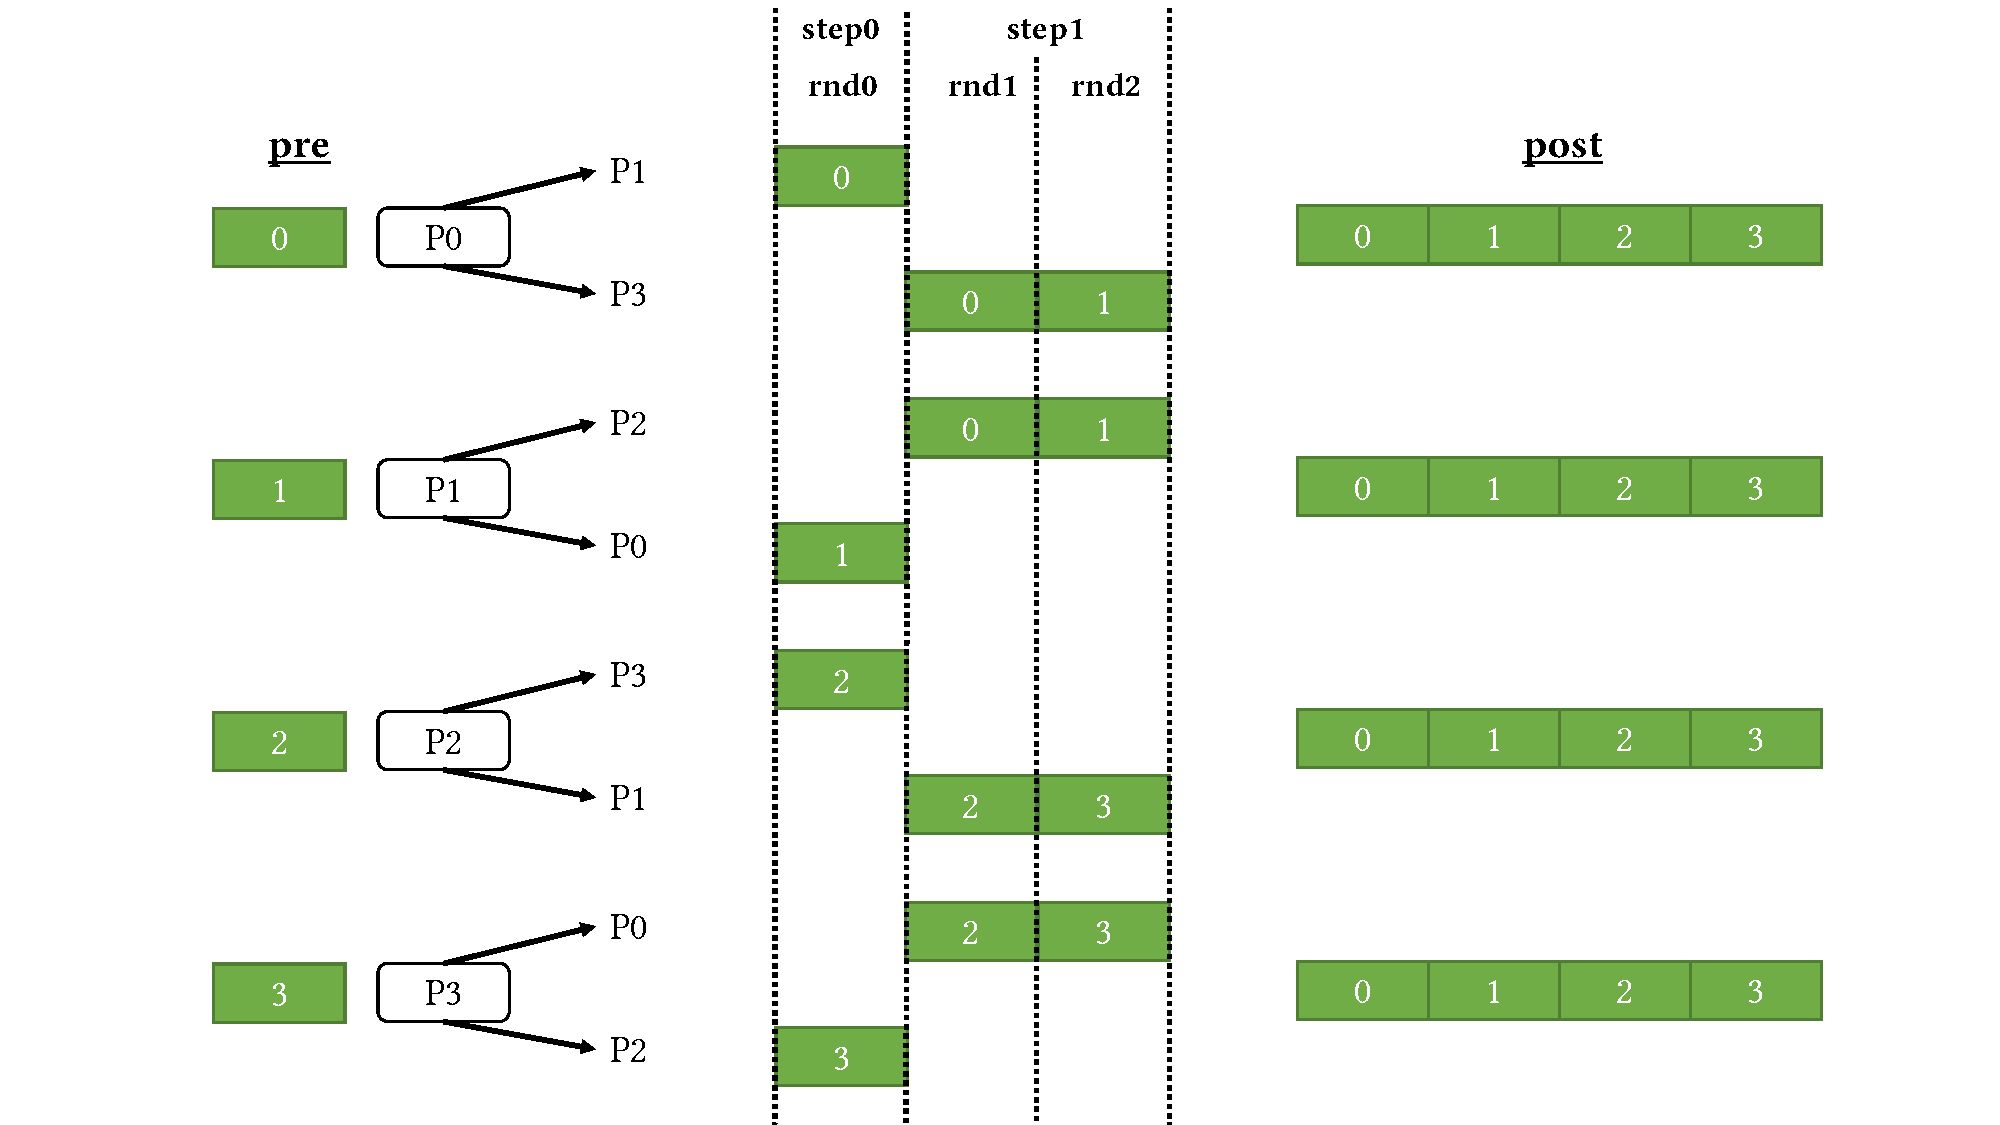
\includegraphics[width=\columnwidth]{figures/allgatherex.pdf}
    \caption{A $1$-synchronous algorithm for \allgather on a ring topology.}
    \label{fig:allgatherex}
\end{figure}

Figure~\ref{fig:allgatherex} shows the
recursive-doubling~\cite{thakur2005optimization} algorithm for
\allgather for a ring topology of four nodes $P0, P1, P2, P3$ with
four bidirectional links of equal bandwidth. This algorithm proceeds
in two {\em steps}. In the first step, nodes at "distance" 1, namely
$P0, P1$ and $P2, P3$ send their data to each other. Each node now has
data from two nodes, which it communicates entirely with nodes at
distance 2, i.e., nodes $P0, P3$ and $P1, P2$ in the second step. At
the end, each node has data from every other node. Since the second
step involves sending twice the amount of data as the first step, we
say it has two \emph{rounds} where in each round, it sends data. Thus,
this step has a total of $3$ rounds. Of the eight (unidirectional)
links, this algorithm uses only four of them per step. To improve
bandwidth utilization, a better option is to split the input data into
equal-sized {\em chunks} and communicate them independently. For
instance, the ring algorithm described in
Section~\ref{sec:motivation:bw-optimal} uses $3$ chunks per node.

The algorithm in Figure~\ref{fig:allgatherex} and many classical
collective algorithms~\cite{thakur2005optimization,chan2007collective}
are instances of {\em synchronous} algorithms. A synchronous algorithm
proceeds in a sequence of synchronous communication {\em steps} with
nodes waiting for other nodes to finish their rounds before starting
the next step. Even if an implementation might not enforce a global
barrier across the nodes, these algorithms choose the amount of data
to communicate per step based on the bandwidth constraints so that the
nodes finish each step at (roughly) the same time.

Many algorithms, like the one in Figure~\ref{fig:allgatherex},
communicate different numbers of chunks per step. We consider each
step as consisting of multiple rounds with each node sending at most
one chunk per unit-bandwidth on its outgoing links. Intuitively, the
number of rounds in an algorithm controls its bandwidth cost, while
the number of steps controls its latency cost. A synchronous algorithm
with $\steps$ steps and $\rounds$ rounds is {\em $k$-synchronous} if
$\rounds \leq \steps + k$. The parameter $k$ limits the amount of
communication per step and allows an SMT solver to effectively search
the space of algorithms bounded by that $k$.
%\todo{Madan mentioned in the chat that for a given $k$, we use it to
%bound $R$. We can make it clearer. The first time I read this, I
%thought we are changing $k$ for some $R$ and $S$ such that $k$ is the
%smallest number such that $R\le S+k$.}

%The terminology of steps and rounds might be confusing at first. The
%best way to distinguish them is to note that in the $(\alpha, \beta)$
%cost model, the latency cost of a $k$-synchronous algorithm depends
%on the number of steps, while the bandwidth cost depends on the
%number of rounds and the number of the chunks.

\subsection{Non-Combining Collective Instance}
Now we will provide a uniform formulation for representing
$k$-synchronous algorithms for \broadcasting collectives. An instance
of \collectiveproblem is a tuple
$(\gchunk,\steps,\rounds,\size,\bw,\pre,\post)$, where
\begin{itemize}
    \item[] \hspace{-0.5cm}Parameters:
    \begin{itemize}
    \item $\gchunk\in\posint$ is the global number of chunks
    \item $\steps\in\posint$ is the total number of steps
    \item $\rounds\in\posint$ is the total number of rounds
    \end{itemize}
    \item[] \hspace{-0.5cm}Topology:
    \begin{itemize}
    \item $\size\in\posint$ is the number of nodes
    \item
    $\bw\subseteq\powerset(\range{\size}\times\range{\size})\times\mathbb{N}$
    is the bandwidth relation
    \end{itemize}
    \item[] \hspace{-0.5cm} Specification:
    \begin{itemize}
        \item $\pre\subseteq\range{\gchunk}\times\range{\size}$ is the
        pre-condition
        \item $\post\subseteq\range{\gchunk}\times\range{\size}$ is
        the post-condition
    \end{itemize}
\end{itemize}
Note that for a set $M$ we write $\powerset(M)$ for the power set of
$M$, i.e., the set of all subsets. For an integer $x$, we write
$\range{x}$ for the set $\{0, 1, \ldots, x\}$. Here, $\gchunk, \steps,
\rounds$ are parameters to the desired $k$-synchronous algorithm. The
rest are explained below.

\subsubsection{Topology}
\label{sec:topology}
$\size$ is the number of nodes in the topology. $\bw$ gives a flexible
way to express different bandwidth constraints we have seen in
practice. In its most general form, $\bw$ bounds the sum of chunks
sent along a set of edges in a single round. A point-to-point
communication link from $s$ to $d$ with maximum bandwidth (in chunks
per round) $b$ can be modeled by $(\{(s, d)\}, b) \in \bw$. Some
topologies might limit the net outgoing bandwidth $b$ from a certain
node $s$. If $E$ is the set of outgoing neighbors of $s$, we can model
this by $(\{(s, e) \mid e \in E\}, b) \in \bw$. To model shared bus
topologies, where only one node can send in a round, we include
$(\{(a, b) \mid a \in N, b \in N\}, b)$ in $\bw$ for the set of nodes
$N$ sharing the same link. Note that these constraints are per round,
and when performing $r_i$ rounds in step $i$, we simply multiply the
bandwidth constraint by $r_i$.

\newcommand{\relAll}{All\xspace}
\newcommand{\relRoot}{Root\xspace}
\newcommand{\relScattered}{Scattered\xspace}
\newcommand{\relTranspose}{Transpose\xspace}
\newcommand{\chunkReduce}{\left\lfloor\frac{i}{\size}\right\rfloor}

\subsubsection{Collective specification}
\label{sec:specifications}
The $\pre$ relation specifies the nodes where the chunks reside at the
beginning of the algorithm and the $\post$ relation specifies the set
of nodes where a chunk needs to be transferred to.
Table~\ref{tbl:relations} specifies useful relations that can be used
to specify common collectives as shown in Table~\ref{tbl:collectives}.
For instance, \allgather starts in a state where chunks are in the
\relScattered relation in Table~\ref{tbl:relations}. In other words,
the $c$ chunks of the input at node $n$ are given chunk identifier
$i\cdot P + n$ for $0 \leq i < c$. From this \relScattered state,
\allgather requires all the input chunks to be copied to all nodes, as
specified by \relAll relation in Table~\ref{tbl:relations}. Similarly,
\broadcast requires all the chunks from the root $n_{root}$ to be
copied to all nodes.

\begin{comment}
We have identified a small number of relations
(Table~\ref{tbl:relations}) that can be mixed-and-matched to model
most common collective primitives (Table~\ref{tbl:collectives}).
Collectives using \relRoot require that a root node $n_\mathit{root}$
has been given. The \relScattered relation is used in collectives that
evenly distribute input data onto nodes, and collectives that use it
require that $\chunk\bmod\size=0$ The \relTranspose relation is used
in conjunction with \relScattered to re-distribute scattered data, and
to ensure an even redistribution these collectives require that
$\chunk\bmod\size^2=0$.

\allreduce as it is specified in Table~\ref{tbl:collectives} needs an
associative reduction operation or else it can give different results
on different nodes. See Section~\ref{sec:background-collectives} for
more discussion.
\todo{Point this Section reference to where the allreduce discussion actually ends up at.}
\end{comment}

\begin{comment}
nodes each identifier starts from, while $\post$ specifies the nodes
that each identifier must end up on. For example, a point-to-point
send primitive with $\size=2$ and $\chunk=1$ might have
$\pre=\{(0,0)\}$ and $\post=\{(0,1)\}$. Note that the pre-condition
can specify that copies of an identifier start from multiple nodes,
which is not useful for traditional collectives. However, this feature
can be useful for specifying more exotic collectives for situations
where an application has already placed identical copies of data onto
some nodes.
\end{comment}

\begin{comment}
% Madan moved this to earlier

The bandwidth relation $\bw$ gives a flexible way to express various
kinds of networks. Topologies with direct links between a source node
$s$ and a destination node $d$ will have $\bw$ of the form
$\{(\{(s,d)\},b),(\{(s',d')\},b'),\dotscend\}$, where $b,b',\dotscend$
give the per link bandwidths. And, to limit the total outgoing
bandwidth from a node $n$ to be no more than $b$, may be modeled with
an entry of the form $(\{(n,n') \setwhere n'\in\range{\size}\},b)$. A
switch that all traffic between two sets of nodes $P$ and $Q$ can be
modeled with an entry of the form $(\{(n,n') \setwhere n\in P \wedge
n'\in Q\},b)$. See Section~\ref{sec:topologies} for details on how we
model the network topologies found in our hardware targets.
\end{comment}

\begin{comment}
The qouta relation $\qouta$ allows multiple chunks be sent in a step
through a link. A link with a bandwidth of $b$ can transfer $2b$
chunks in a 2 short steps which each transferring $b$ chunks but
alternatively the same link could transfer $2b$ chunks in a longer
step. This enables the synthesizer to find algorithm which are more
latency optimal.
\todofor{Olli}{Do we want to talk about sharing of nodes here? - this is important as most cross node topologies have shared interconnects in addition to PCIe}
\todofor{Olli}{our assumptions below  do not allow different sized chunks.  this is fine, but i wonder if we want to have a section on our ``asusmptions'' to push off potential challenges from reviewers.}
\end{comment}

\begin{comment}
% Madan: changed the example to allgather
As an example, consider the \reduce collective primitive, which
reduces data from all nodes onto a single root node $n_\mathit{root}$.
The target hardware will have some number of nodes $\size$ and
bandwidth relation $\bw$. To split the input data into $d$ chunks, the
number of identifiers is set to $\chunk=d*\size$. Now the problem of
synthesizing an algorithm can be modeled by setting:
\begin{align*}
    \pre&=\{(c,n)\in\range{\chunk}\times\range{\size} \setwhere n=c\bmod \size\} \\
    \post&=\range{\chunk}\times\{n_\mathit{root}\} \\
    \chunk(i)&=\left\lfloor\frac{i}{\size}\right\rfloor
\end{align*}
The pre-condition requires that identifiers are distributed onto nodes
in a round-robin fashion, while the post-condition requires all
identifiers to end up on the root node. $\chunk$ maps blocks of
$\size$ identifiers to the same chunk, thus reducing them together in
the result.
\end{comment}


\begin{table}[bp]
    \center
    \caption{Common relations in pre- and post-conditions of collective primitives.}
    \begin{tabularx}{\columnwidth}{@{}Xl@{}}
        \toprule
        Name & Relation \\
        \midrule
        \relAll & $\range{\gchunk}\times\range{\size}$ \\
        \relRoot & $\range{\gchunk}\times\{n_\mathit{root}\}$ \\
        \relScattered & $\{(c,n)\in\range{\gchunk}\times\range{\size}
        \setwhere n=c\bmod \size\}$ \\
        \relTranspose & $\{(c,n)\in\range{\gchunk}\times\range{\size}
        \setwhere n=\left\lfloor\frac{c}{\size}\right\rfloor\bmod
        \size\}$ \\
        \bottomrule
    \end{tabularx}
    \label{tbl:relations}
\end{table}
\begin{table}[bp]
    \caption{Specifications of collective primitives.}
    \begin{tabularx}{\columnwidth}{@{}Xll@{}}
        \toprule
        Collective & $\pre$ & $\post$ \\
        \midrule
        \gathercoll & \relScattered & \relRoot  \\
        \allgather & \relScattered & \relAll  \\
        \alltoall & \relScattered & \relTranspose  \\
        \broadcast & \relRoot & \relAll \\
        \scatter & \relRoot & \relScattered  \\
        \bottomrule
    \end{tabularx}
    \label{tbl:collectives}
\end{table}

While \collectiveproblem uses a global number of chunks $\gchunk$, it
is more typical in existing literature to consider the per-node number
of chunks $\chunk$. We will use the per-node number when discussing
the cost model and search algorithm in Sections~\ref{sec:costmodel}
and \ref{sec:pareto:optimal} and when presenting our evaluation in
Section~\ref{sec:evaluation}. Note that how these two counts relate to
each other is collective dependent: for \broadcast $\gchunk=\chunk$,
while for \allgather $\gchunk=\size\cdot\chunk$. The formalization
must still use a global numbering of chunks, as some exotic
collectives, e.g. MPI's Allgatherv, may not have a single per-node
chunk count.

\subsection{Candidate Solution}
Given an instance of \collectiveproblem
$(\gchunk,\steps,\rounds,\size,\bw,\pre,\post)$, a candidate solution
is a pair $(\rparts,\sends)$. Here $\rparts$ is a sequence
$r_0,\allowbreak r_1,\allowbreak \dotsc,\allowbreak r_{\steps -1}$
such that $\sum_i r_i = \rounds$ and denotes the number of rounds per
step. $\sends$ is a set of sends of the form $(c,n,n',s)$, which
specifies that chunk $c$ must be sent from node $n$ to node $n'$ at
step $s$. This defines a {\em run} defined as a  sequence
$V_0,V_1,\dotsc,V_{\steps}$ such that $V_0 = \pre$ and for all $0 \leq
s < \steps$, $V_{s+1}$ reflects the chunks present at a given node
after accounting for the sends at step $s$:
%$V_{\steps -1} \subseteq \post$
$$ V_{s+1} = V_{s} \cup \{(c,n') \mid (c, n) \in V_{s} \wedge (c, n,
n', s) \in \sends\} $$

This candidate solution is a valid $k$-synchronous algorithm for the
instance if $V_{\steps} \subseteq \post$ and the following bandwidth
constraint hold
\begin{align*}
    &\begin{aligned}
        \forall &s\in\range{\steps},\,(L,b)\in\bw \qst, |\{(c,n,n',s)\in \sends \setwhere (n,n')\in L\}|\leq b \cdot r_s
    \end{aligned}
\end{align*}
%\todo{introduce in the order of correctness constraints and bandwidth
%constraints. Sequence $Q$ can be explained together with the
%bandwidth constraints}
At each step $s$ consisting of $r_s$ rounds, the number of sends in
each link should be bounded by the bandwidth constraint multiplied by
$r_s$.
% \begin{align*} & \exists r_0, r_1, \ldotsc, r_{\steps-1} : \sum_i
%     r_i = \rounds \wedge \\
%     & \forall &t\in\range{\steps},\,(L,b)\in\bw \qst \\
%     & |\{(c,n,n',t)\in S \setwhere (n,n')\in L\}| \leq b \cdot r_i
% \end{align*}

\begin{comment}
\begin{align*}
    &V_0=\{(i,n,\Ite{(i,n)\in\pre}{1}{0}) \setwhere (i,n)\in\range{\chunk}\times\range{\size}\} \\
    &\begin{aligned}
        V_t=\{(i,n,\Sigma\{&r' \setwhere (i,n',r')\in V_{t-1} \wedge (n=n' \vee \\
        &(\chunk(i),n',n,t-1)\in S)\}) \setwhere (i,n)\in\range{\chunk}\times\range{\size}\}
    \end{aligned}
\end{align*}
Each $V_t$ has entries of the form $(i,n,r)$, which indicate that
identifier $i$ has reached node $n$ a total of $r$ times.
%
The candidate solution $S$ is an \emph{algorithm} for $P$ if and only
if the following conditions hold:
\begin{alignat}{3}
    &\mathrlap{ \forall (i,n,r)\in V_{\steps} \qst (i,n)\in\post
    \Rightarrow r=1} \tag{A1}\label{eqn:a1}\\
    &\begin{aligned} \forall &t\in\range{\steps},\,(L,b)\in\bw \qst \\
        &b\geq|\{(c,n,n',t)\in S \setwhere (n,n')\in L\}|
    \end{aligned} \tag{A2}\label{eqn:a2}
\end{alignat}
Condition~\ref{eqn:a1} ensures that the algorithm satisfies the
post-condition of the problem instance. Because reduction operations
are not always idempotent, Condition~\ref{eqn:a1} requires that each
identifier has contributed to the result exactly once.
Condition~\ref{eqn:a2} ensures that the bandwidth limitations are
respected by counting the number of sends happening on each time step
and checking that this is below the limit. Because we assume that all
chunks are the same size, \ref{eqn:a2} can simply compare the number
of sends to the bandwidth limit.
\end{comment}
%\subsection{Specifications for Common Collectives}
%\label{sec:specifications}


\subsection{SMT Encoding for Non-Combining Collectives}
\label{sec:encoding}
\begin{comment}
    While \collectiveproblem is amenable to a direct encoding into
    SMT, we choose to use an encoding for the special case of
    $\gchunk(i)=i$, i.e., the case where there is no reduction
    happening and each identifier corresponds to a unique chunk. We
    call these collectives \emph{broadcasting collectives}.
    Section~\ref{sec:reduction} will then show how the synthesis
    problem for a larger class of collectives that do perform
    reduction can be reduced to the synthesis problem for broadcasting
    collectives. The reduction reduces the number of identifiers,
    leading to better synthesis performance. Since we assume that
    $\gchunk(i)=i$ we use chunks and identifiers interchangeably in
    the following explanation.
\end{comment}
Given an instance, the SMT encoding incorporates the constraints above
allowing the SMT solver to systematically search over candidate
solutions $(\rparts, \sends)$. It is straightforward to encode each
$r_s$ of $\rparts$ as integer variables whose sum is $\rounds$. In
contrast, one has to be careful in encoding $\sends$. For instance,
our initial attempt to encode every tuple $(c, n, n', s) \in \sends$
as a Boolean variable was not successful, because Z3, the SMT solver
we used, did not solve larger problem instances fast enough. One way
we were able to scale Z3 is to use a careful combination of Boolean,
integer, and pseudo-Boolean constraints as we describe below.

We split the encoding of $\sends$ into integer variables $\start{c}{n}
\geq 0$, indicating the earliest step a chunk $c$ becomes available at
node $n$ and Boolean variables $\send{n}{c}{n'}$ determining whether a
node $n$ sends chunk $c$ to $n'$ (at any step).
\newcommand{\edges}{E}
To help with pruning the encoding, let $\edges=\{(n,n') \setwhere
\allowbreak \forall (L,b)\in\bw \qst (n,n')\in L \Rightarrow b > 0\}$,
i.e., the pairs of nodes with non-zero bandwidth between them.
Pseudo-Boolean constraints allow one to use Boolean variables as $0,1$
integers which we will use in the exposition below.

The following two constraints enforce the pre- and post-conditions.
%Now we describe the constraints required for the encoding. Chunks
%must have a starting time of zero on all associated nodes in the
%pre-condition. For each $(c,n_{\mathit{pre}})\in\pre$ add the
%following constraint:
\begin{align}
%    \forall (c,n) \in \range{\gchunk} \times \range{\size} (c,n) \in \pre &\equiv \start{c}{n}=0
    \forall (c,n) \in \pre \ \ \start{c}{n} &=0
    \tag{E1}\label{eqn:bc-zero} \\
    \forall (c,n) \in \post \ \ \start{c}{n}&\leq \steps
%    \start{c}{n_{\mathit{post}}}&\leq\steps
    \tag{E2}\label{eqn:bc-insteps}
\end{align}
If a chunk becomes available in a node, but is not part of the
precondition, then the node should have received the chunk from some
other node. For optimality, we also enforce that the node does not
redundantly receive the chunk more than once.
%For each $(c,n)\in(\range{\ids}\times\range{\size})\setminus\pre$ add
%the following constraint:
\begin{align}
    \forall (c,n) \not\in \pre \ \ \start{c}{n}&\leq \steps \Rightarrow \Sigma_{(n',n)\in\edges}\,\send{n'}{c}{n}=1
    \tag{E3}\label{eqn:bc-hassender}
\end{align}
To send a chunk, it must exist on the source node before it is
received on the destination node.
%For each chunk $c\in\range{\ids}$ and pair of connected nodes
%$(n,n')\in\edges$ add the following constraint:
\begin{align}
    \forall (c,n) \in E \ \ \send{n}{c}{n'}\Rightarrow\start{c}{n}<\start{c}{n'}
%    \send{n}{c}{n'}\Rightarrow\start{c}{n}<\start{c}{n'}
    \tag{E4}\label{eqn:bc-sendexisting}
\end{align}
%Constraints \ref{eqn:bc-zero}, \ref{eqn:bc-insteps},
%\ref{eqn:bc-hassender} and \ref{eqn:bc-sendexisting} would be
%sufficient to satisfy Condition~\ref{eqn:a1}.
The following enforces the bandwidth constraint at all steps $1 \leq s
\leq \steps$ and bandwidth constraint $(L,b)\in\bw$.
%To satisfy Condition~\ref{eqn:a2}, we must ensure that the bandwidth
%limitations of the topology are respected. For each step of the
%algorithm $1 \leq t \leq \steps$ and bandwidth constraint
%$(L,b)\in\bw$ add the constraint:
\begin{align}
    \Sigma_{(c,(n,n'))\in\range{\gchunk}\times L}\left(\send{n}{c}{n'}\wedge\start{c}{n'}=s\right)\leq b \cdot r_s
    \tag{E5}\label{eqn:bc-bw}
\end{align}
%
Note, we have multiplied the bandwidth constraints by $r_s$ to allow
$r_s$ rounds at step $s$.
%
Finally, the following bounds the total rounds $\rounds$.
\begin{align}
    \Sigma_{1\leq s\leq\steps}(r_s)=\rounds
    \tag{E6}\label{eqn:bc-rounds}
\end{align}

%\begin{comment}
Once the problem instance has been encoded, the SMT solver will
attempt to find a model $M$, which maps the variables $\start{c}{n}$,
$\send{n}{c}{n'}$ and $r_s$ to concrete values such that Constraints
\ref{eqn:bc-zero} through \ref{eqn:bc-rounds} are satisfied. If a
model exists then an algorithm $(\rparts, \sends)$ can be constructed
with:
\begin{align*}
    \rparts&=M(r_0),\dotsc,M(r_{\steps-1}) \\
    \sends&=\{(c,n,n',t) \setwhere M(\send{n}{c}{n'}) \wedge M(\start{c}{n}) = t+1 \}.
\end{align*}
If the SMT solver says the problem is unsatisfiable, then no algorithm
exists for the problem instance.
%\end{comment}


\subsection{\reducingCap Collectives}
\label{sec:reduction}
It is well known that certain \reducing collectives are {\em inverses}
of \broadcasting collectives. For instance, a \reduce algorithm can be
generated by inverting an algorithm for \broadcast on a topology where
all links have been reversed. Intuitively, whenever the \broadcast
sends the same chunk to two different nodes, in its inverse the
\reduce algorithm will receive the two {\em versions} of the chunk
from these nodes and apply the reduction operation. The node will send
the resulting chunk to the node it received the chunk from in the
\broadcast. Similarly, we can generate \reducescatter algorithms by
inverting \allgather algorithms. %For space reasons, we do not
describe the formal procedure of inverting \broadcasting collectives.

Generally the inverting procedure works for any \reducing collective
that has a single root node for each chunk. Notably, this does not
include \allreduce, which replicates the result onto all nodes. For
synthesizing \allreduce algorithms, we first notice that \allreduce
can be expressed as a combination of \reducescatter followed by an
\allgather. We synthesize \allreduce algorithms by synthesizing an
\allgather algorithm and preceding it with its inverse \reducescatter
algorithm.

\begin{comment}
While the SMT encoding presented in the previous section could be
extended to handle the general case, a direct encoding would require
tracking staring times per-identifier instead of per-chunk. For the
reducing collectives in Section~\ref{sec:specifications} this would
inflate the number of $\start{i}{n}$ variables by a factor of $\size$.
However, it turns out that for a class of reducing collectives that
reduce each chunk onto a unique node the synthesis problem can be
reduced to the subclass for broadcasting collectives. The special case
of turning an algorithm for \allgather into one for \reducescatter
with a symmetric bandwidth relation is well-known. This section
presents a generalized reduction, that handles any collective in this
class on any kind of topology.

\newcommand{\chunktochunk}{\mathcal{T}}
\newcommand{\algtoorig}{\mathcal{R}}

The reduction involves transforming pre- and post-con\-di\-tions such
that there is one identifier for each unique chunk. Given any post- or
pre-condition $R$, we use the following function to perform this
transformation:
\[
    \textstyle
    \chunktochunk(R) = \{(c,n) \setwhere \exists (i,n)\in R \qst \chunk(i)=c \}
\]
Let $P=(\size,\bw,\chunk,\chunk,\pre,\post,\steps)$ be an instance of
\collectiveproblem such that the following condition holds:
\begin{gather}
    % \chunk\bmod\size=0 \tag{R1}\\
    % \chunk(i)=\chunkReduce \tag{R2}\\
    \forall (i,n),(i',n')\in\post \qst \chunk(i)=\chunk(i') \Rightarrow n=n' \tag{SR}\label{eqn:single-root}
\end{gather}
Out of the collectives in Table~\ref{tbl:collectives} this condition
holds for \reduce and \reducescatter, but not for \allreduce. The
reason is that the post-condition is required to give a unique root
node for each set of identifiers that correspond to the same chunk,
but \allreduce reduces each chunk onto all nodes.

Additionally, without loss of generality, we assume that the set of
chunks $\{\chunk(i) \setwhere i\in\range{\chunk}\}$ forms a continuous
integer interval starting from zero. Any $P$ not satisfying this can
be transformed to this form by remapping $C$.

Now construct a new instance of \collectiveproblem as
$P'=(\size,\allowbreak\bw',\allowbreak\chunk',\allowbreak\chunk',\allowbreak\pre',\allowbreak\post',\allowbreak\steps)$
where:
\begin{gather*}
    \bw'=\{(L',b) \setwhere (L,b)\in\bw \wedge L'=\{(n',n) \setwhere (n,n')\in L\} \} \\
    \chunk'=|\{\chunk(i) \setwhere i\in\range{\chunk}\}| \hspace{2em} \chunk'(i)=i \\
    \post'=\chunktochunk(\pre) \hspace{2em} \pre'=\chunktochunk(\post)
\end{gather*}
Let $\algtoorig$ be a function for mapping algorithms for $P'$ back to
$P$ defined as follows:
\[
    \algtoorig(S')=\{ (c,n',n,\steps-t-1) \setwhere (c,n,n',t)\in S' \}
\]
\begin{theorem}
    Given an algorithm $S'$ for $P'$, the transformed solution
    candidate $S=\algtoorig(S')$ is an algorithm for $P$.
    \label{thm:reduction-solution}
\end{theorem}
    \begin{proof}
    % A sequence of sends
    % $(a_0,n_0,n'_0,t_0),\dotsc,(a_{m-1},n_{m-1},n'_{m-1},t_{m-1})$
    % in a solution candidate is a \emph{path} (of length $m$) if
    % $\forall i\in\range{m} \qst $

    Given an identifier $i$ the sequences of nodes $n_0,\dotsc,n_m$
    and steps $t_0,\dotsc,t_{m-1}$ form a \emph{path} from $n_0$ to
    $n_m$ in a solution candidate $S''$ if $\forall k\in\range{m} \qst
    (\chunk(i),n_k,n_{k+1},t_k)\in S''$ and $\forall k\in\range{m-1}
    \qst t_k < t_k+1 \wedge 0 \leq t_k \leq \steps-1$.

    %There is a unique starting node for each chunk in $P'$.
    Because \ref{eqn:single-root} holds for $P$, then for each
    identifier $i\in\range{chunks}$ there exists a unique
    $(i,n_{\mathit{root}})\in\post$ and thus, due to the way
    $\chunktochunk$ collapses identifier of the same chunk into a
    single identifier, a unique
    $(\chunk(i),n_{\mathit{root}})\in\pre'$. Now since \ref{eqn:a1}
    holds for $S'$, for each $(i,n)\in\post'$ there exists a unique
    path from $n_{\mathit{root}}$ to $n$ in $S'$, as otherwise the
    count for $(i,n)$ in $V'_\steps$ would not be 1.

    Due to the way $\algtoorig$ flips the sources and destinations of
    sends and also reverses their ordering in time, each path in $S'$
    from a node $n$ to another node $n'$ corresponds to a path from
    $n'$ to $n$ in $S$. Thus for each $(i,n)\in\pre$ there exists a
    unique path from $n$ to $n_{\mathit{root}}$. Therefore,
    \ref{eqn:a1} holds for $S$.

    Because \ref{eqn:a2} holds for $S'$ and both $\bw'$ and
    $S=\algtoorig(S')$ flip the order of sources and destinations,
    then \ref{eqn:a2} holds also for $S$, which therefore is an
    algorithm for $P$.
\end{proof}

\begin{theorem}
    If no algorithm exists for $P'$ then there are no algorithms for
    $P$ either.
    \label{thm:reduction-no-solution}
\end{theorem}
    The proof for Theorem~\ref{thm:reduction-no-solution} takes a
    similar form to the proof for
    Theorem~\ref{thm:reduction-solution}.
\begin{proof}
    Assume there exists an algorithm $S$ for $P$. Since \ref{eqn:a1}
    holds for $S$, for each $(i,n)\in\pre$ there exists a unique path
    from $n$ to $n_{\mathit{root}}$ (see proof of
    Theorem~\ref{thm:reduction-solution} for explanation of
    $n_{\mathit{root}}$).

    Let $S'=\algtoorig(S)$. Given that $\algtoorig$ flips sources and
    destinations of sends as well as reverses their stepwise ordering,
    each path in $S$ corresponds to a reversed path in $S'$. Thus for
    each $(i,n)\in\post'$ there exists a unique path from
    $n_{\mathit{root}}$ to $n$. Therefore, \ref{eqn:a1} holds for $S'$

    Because \ref{eqn:a2} holds for $S$ and both $\bw'$ and
    $S=\algtoorig(S')$ flip the order of sources and destinations,
    then \ref{eqn:a2} holds also for $S'$, which therefore is an
    algorithm for $P$. This is a contradiction. Thus the assumption
    that $S$ is an algorithm for $P$ is false and the original theorem
    is true.
\end{proof}

Now for any instance of \collectiveproblem for which
\ref{eqn:single-root} holds this reduction can be used to transform it
into a form that the SMT encoding in Section~\ref{sec:smt-encoding}
can be used. If a solution exists then $\algtoorig$ can be used to get
a solution to the original instance. If no solution exists, then there
is no solution to the original instance either.
\end{comment}

\subsection{Cost Model}
\label{sec:costmodel}
Say we have synthesized a $k$-synchronous algorithm with $\chunk$
chunks, $\steps$ steps, and $\rounds$ rounds. We will use the
$(\alpha, \beta)$ cost model~\cite{hockney1994communication} to
evaluate cost of this algorithm. Here, $\alpha$ is the latency of each
link in the topology and $\beta$ is the time taken sending a byte
along a unit-bandwidth link. If the input data of $L$ bytes is divided
into $\chunk$ chunks, a step $s$ with $r_s$ rounds takes $\alpha +
\frac{r_s}{\chunk}\cdot L \cdot \beta$ time. Therefore, the entire
algorithm will finish in time
$$ \steps \cdot \alpha + \frac{\rounds}{\chunk} \cdot L \cdot \beta. $$
%In effect, one can reduce the latency cost by reducing the number of
%steps, and reduce the bandwidth cost either by increasing the number
%of chunks or decreasing the number of rounds.

\subsection{Pareto-optimal Algorithms}
\label{sec:pareto:optimal}
The discussion above shows that for a given topology and a collective
with an input size $L$, the cost of a $k$-synchronous algorithm can be
characterized by the tuple $(\steps, \frac{\rounds}{\chunk})$. An
algorithm with cost $(a,b)$ is {\em Pareto-optimal} with respect to
the class of $k$-synchronous algorithms if for every algorithm in this
class with cost  ($a', b')$ we have $a = a' \Rightarrow b' \geq b$ and
$b = b' \Rightarrow a' \geq a$. An algorithm with cost $(a,b)$ is
considered {\em latency-optimal} ({\em bandwidth-optimal}), if for
every $k$-synchronous algorithm with cost $(a',b')$ we have $a' \geq
a$ ($b' \geq b$).

Note that latency- or bandwidth-optimal algorithms are not necessarily
Pareto-optimal as they can be "wasteful" in the other parameter.
Pareto-optimal algorithms form a {\em Pareto-frontier} with different
algorithms in the frontier being better than others for a given input
size $L$ based on the $\alpha$ and $\beta$ parameters of the topology.

Algorithm~\ref{alg:pareto} systematically synthesizes Pareto-optimal
$k$-synchronous algorithms. The inputs are the parameter $k$, the name
of the collective to synthesize, and the topology parameters $\size,
\bw$~(Section~\ref{sec:topology}). The procedure computes the latency
lower bound $a_l$ from the diameter of the topology, and the bandwidth
lower bound $b_l$ from the inverse bisectional bandwidth of the
topology. The procedure starts enumerating steps $\steps$ starting
with $a_l$. Then it generates $A$, the candidate set of tuples
$(\rounds, \chunk)$ that satisfy the round constraint and the inverse
bandwidth constraint. Note that without the $k$ parameter, this set
would be unbounded. The procedure checks if a
$(\steps,\rounds,\chunk)$ algorithm exists in the increasing order of
the bandwidth cost $\frac{\rounds}{\chunk}$ using the encoding
discussed in Section~\ref{sec:encoding}. If one exists, the reported
algorithm is guaranteed to be Pareto-optimal for the current steps
$\steps$. As we increase the number of $\steps$, we get algorithms
with lower bandwidth cost. Additionally, if the current bandwidth cost
matches the lower bound $b_l$, the procedure returns. As we have
already generated the Pareto-optimal algorithm with $b_l$ bandwidth
cost, it is not necessary to increase $\steps$ further. Note, that it
is possible for this procedure to never terminate as there can
sometimes be unbounded number of Pareto-optimal algorithms for certain
topologies and collectives. While the synthesis procedure above is for
\broadcasting collectives, synthesis for \reducing collectives is
similar~(Section~\ref{sec:reduction}).
%\todo{explains that when increase $S$, we should have better $(R,C)$
%pairs for better bandwidth. The limit the to the bandwidth is the
%lower bound, once we can reach it, there's no point increasing $S$,
%because it increases the latency.}


\begin{algorithm}
	\caption{Synthesizing Pareto-Optimal Algorithms}
    \label{alg:pareto}
    \begin{algorithmic}[1]
        \Procedure{Pareto-Synthesize}{$k, \mathit{Coll}, \size, \bw$}
        \State $a_l = \mathit{Diameter(\size, \bw)}$ \State $b_l =
        \mathit{InvBisectionBandwidth(\size, \bw)}$ \State $(\pre,
        \post) = \mathit{Lookup(Coll)}$
        \Comment{Table~\ref{tbl:collectives}} \For
        {$\steps=a_l,a_l+1\ldots$} \State $A = \{(\rounds,\chunk) \mid
        \steps \leq \rounds \leq \steps+k \wedge
        \frac{\rounds}{\chunk} \geq b_l\}$ \For {$(R,\chunk) \in A$ in
        ascending order of $\frac{R}{\chunk}$} \State
        $\gchunk=\toglobal(\mathit{Coll},\chunk)$ \If
        {$\mathit{SMT(\gchunk, \steps, \rounds, \size, \bw, \pre,
        \post) = SAT}$} \State Report synthesized algorithm
        $(\steps,\rounds,\chunk)$ \If {$\frac{\rounds}{\chunk} = b_l$}
        \State {\bf return} \EndIf \State {\bf break} \EndIf \EndFor
        \EndFor \EndProcedure
	\end{algorithmic}
\end{algorithm}
